\section{Experiment 3}\label{sec:experiment-3}
This experiment is targetted towards exploring the differences in the kernels that have been implemented in cross-validation regarding \gls{kpca}. In Experiment~\ref{sec:experiment-1} only the sigmoid kernel was used, and this experiment's goal is to assess whether the choice of kernel could have a major impact the model's performance. The experiment will focus on the confusion matrices and scores obtained from the different kernels. \todo{Is this a good intro? put in Grammarly}


%This is some theory, which should be in Implementation
%As explained in the Chapter Theory, KPCA can have kernels, which will project the data into a higher dimensional feature space, where a hyperplane can be constructed, and perform PCA on it. KPCA does not require the transformation of the inputs into the feature space with the kernel function, but can use the kernels so as to get the dot product of the pair-wise input points~\cite{kpca-book}. The kernels are a measure of similarity between the points~\cite{scikit-learn}, which means that points that are close to each other have higher similarity score, which is computed with the kernel function. The kernels chosen for the experiment are the \gls{rbf} and sigmoid kernels. The sigmoid kernel \textcquote{scikit-learn}{computes the sigmoid kernel between two vectors}, which outputs a value between -1 and 1 for the two given input vectors. The \gls{rbf} kernel \textcquote{scikit-learn}{computes the radial basis function kernel between two vectors}, which outputs a value between 0 and 1.


\subsection{Rules}
The dimensionality reduction methods used in this experiment will be \gls{pca} and \gls{kpca}. The classification method will be \gls{svm}. The kernels used for KPCA will be \gls{rbf} and sigmoid.
The best configuration for each method used in this experiment is shown in Table~\ref{tab:best-configuration-expr-3}. The input of the data samples will be 15000 for both of the methods. The number of components used for all methods will be 49 components. The evaluation will be based on the confusion matrices and the results from the CSV file for cross-validation for \gls{kpca}. The experiment will be run on the pc-2 see hardware specifications in Table~\ref{tab:pc2-specs}.

\begin{table}
    \centering
    \begin{tabular}{lrlll}
        \toprule
        method & components & C & parameter & parameter\\
        \midrule
        PCA-15 & 49 & C = 0.01 &  \\
        KPCA-15 & 49 & C = 1.0 & Gamma = 0.01 & Sigmoid \\
        KPCA-15 & 49 & C = 1.0 & Gamma = 0.001 & RBF \\
        % KPCA-15 & 49 & C = 1.0 & Gamma = 0.001 & Sigmoid \\
        % KPCA-15 & 49 & C = 1.0 & Gamma = 0.01 & RBF \\
        \bottomrule
    \end{tabular}
    \caption{Best configuration for each method used for experiment-3, method-15 means the method with 15 thousand samples.}
    \label{tab:best-configuration-expr-3}
\end{table}

\subsection{Results}\label{subsec:experiment-3-results}
Below is shown the results for the methods. The results are in the form of confusion matrices. Accuracy percentages from the confusion matrices will compare the methods.  

\subsubsection{PCA}
\begin{figure}[htb!]
    \centering
    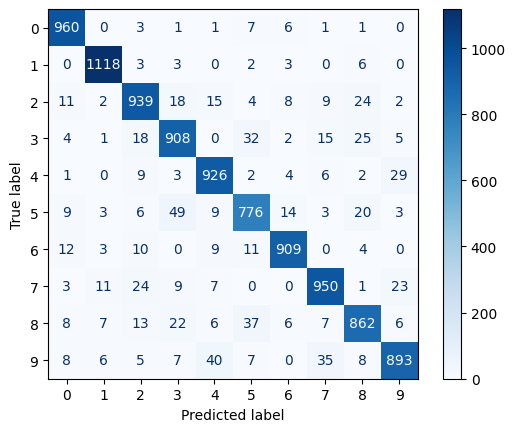
\includegraphics[width=0.8\textwidth]{figures/experiment-3/confusion_matrix_pca_svm.png}
    \caption{Confusion matrix for PCA}
    \label{fig:confusion-matrix-pca-svm}
\end{figure}
Figure~\ref{fig:confusion-matrix-pca-svm} shows the results for \gls{pca}. It has an accuracy of 92.37\%. It shows \gls{pca} is best at recognizing zeros and ones in pictures, as the model had guessed lees on the other numbers when the picture was zero or one. The model has trouble recognizing nines from fours and sevens, threes from fives, and fives from threes and eights.  

\subsubsection{KPCA}
\begin{figure}
    \centering
    \subfloat[\centering Confusion matrix for kPCA Sigmoid]{\label{fig:confusion-matrix-kernel-pca-svm-sigmoid}{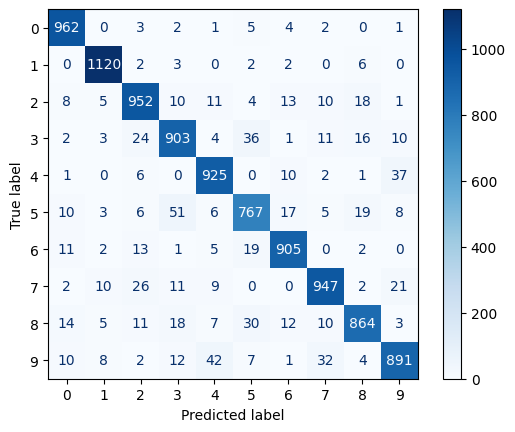
\includegraphics[width=0.45\textwidth]{figures/experiment-3/confusion_matrix_kernel_pca_svm_sigmoid.png} }}
    \qquad
    \subfloat[\centering Confusion matrix for kPCA RBF]{\label{fig:confusion-matrix-kernel-pca-svm-rbf}{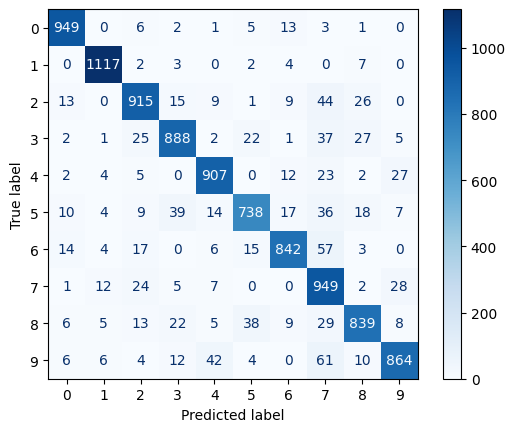
\includegraphics[width=0.45\textwidth]{figures/experiment-3/kernel_pca_rbf_kernel_49.png} }}%
    \caption{both kPCA kernels confusion matrices}
    \label{fig:kpca-kernels}
\end{figure}

Figure~\ref{fig:confusion-matrix-kernel-pca-svm-sigmoid} shows the results for \gls{kpca} with the sigmoid kernel. It has an accuracy of 91.5\%. It shows \gls{kpca-s} is best at recognizing zeros and ones in pictures, as the model had guessed lees on the other numbers when the picture was zero or one. The model has trouble recognizing nines from fours and sevens and tells threes, fives, and eights from each other. 

Figure~\ref{fig:confusion-matrix-kernel-pca-svm-rbf} shows the results for \gls{kpca} with the RBF kernel. It has an accuracy of 89.5\%. It shows \gls{kpca-r} is best at recognizing zeros and ones in pictures, as the model had guessed lees on the other numbers when the picture was zero or one. The model has trouble recognizing nines from fours and sevens and tells fives, threes, and sevens from each other.  

\subsection{Discussion of experiment 3}\label{subsec:discussion-experiment-3}
From the results presented about the differences between the kernels it can be noted that all the methods often confuse the number 9 with 4 and 7; the number 3 with 5 and 7 or 8. It can be further noted that \gls{kpca-r} is the worst at confusing various numbers with the number 7.

\begin{table}[htb!]
    \centering
    \begin{tabular}{lrrrr}
        \toprule
          & pca    & kpca-s & kpca-r \\
        \midrule
        0 & 2.959  & 1.836  & 3.163  \\
        1 & 1.585  & 1.321  & 1.585  \\
        2 & 8.817  & 7.751  & 11.337 \\
        3 & 10.594 & 10.594 & 12.079 \\
        4 & 5.702  & 5.804  & 7.637  \\
        5 & 12.556 & 14.013 & 17.264 \\
        6 & 6.054  & 5.532  & 12.108 \\
        7 & 7.101  & 7.879  & 7.684  \\
        8 & 13.552 & 11.293 & 13.860 \\
        9 & 11.992 & 11.694 & 14.370 \\
        \bottomrule
    \end{tabular}
    \caption{Error percentage for each number for the methods}
    \label{tab:error-percentage-pca-kpca-s-kpca-r}
\end{table}

From the overview provided regarding the difference in numbers, a percentage would be more preferable, more specifically, a percentage of the errors made in the numbers 0-9. The error percentage can be calculated the number of correct predictions divided by the total number of numbers from the given class. Table~\ref{tab:error-percentage-pca-kpca-s-kpca-r} shows the difference in percentages of errors made by the methods for each number.

In Table~\ref{tab:error-percentage-pca-kpca-s-kpca-r} it can be seen that PCA has the best performance for the numbers 4 and 7, while KPCA-S has the best performance for the numbers 2 and 8. PCA and KPCA-S have similar performance for most of the numbers, while KPCA-R has the worst performance for most of the numbers. In parcular, KPCA-R has the worst performance for the numbers 4, 5 and 6, in 6 KPCA-R has a twice as bad score as KPCA-S. 

However, the error percentage is not the only thing that should be considered. The difference between the error percentage between PCA and the two kernel PCA methods, KPCA-S and KPCA-R, is also important. Therefore the difference between the error percentage for the two kernel PCA methods and PCA is presented in Table~\ref{tab:error-percentage-difference-pca-kpca-s-kpca-r}.


The differences between the two kernel PCA methods, KPCA-S and KPCA-R, in relation to the error percentage presented in \gls{pca} is presented in Table~\ref{tab:error-percentage-difference-pca-kpca-s-kpca-r}.

\begin{table}[htb!]
    \centering
    \begin{tabular}{lrrrr}
        \toprule
           & kpca-s & kpca-r    \\
        \midrule
        0  & -1.123  & +0.204   \\
        1  & -0.264  & 0        \\
        2  & -1.066  & +2.52    \\
        3  &  0      & +1.485   \\
        4  & +0.102  & +1.935   \\
        5  & +1.457  & +4.708   \\
        6  & -0.522  & +6.054   \\
        7  & +0.778  & +0.583   \\
        8  & -2.259  &  +0.308  \\
        9  & -0.298  & +2.378   \\
        \bottomrule
    \end{tabular}
    \caption{Difference between the error percentage for the kernels compared to pca. The difference is calculated by subtracting the error percentage of the kernel from the error percentage of pca.}
    \label{tab:error-percentage-difference-pca-kpca-s-kpca-r}
\end{table}

Based on the tables~\ref{tab:error-percentage-pca-kpca-s-kpca-r} and \ref{tab:error-percentage-difference-pca-kpca-s-kpca-r} it seems as if \gls{kpca-r} predicts too many times the number 7 for various numbers, which is a reason for why \gls{kpca-s} is better than \gls{kpca-r}.


%In Section~\ref{subsec:experiment-3-results}, the results were presented for the different \gls{kpca} kernels, along another hyperparameter, the $\gamma$ value. Whether the $\gamma$ value has an effect on the accuracy of the \gls{kpca} method (while preserving the other hyperparamters) can be looked up in the CSV file. Their results can be seen in Table~\ref{tab:gamma-values-kpca}.

% \begin{table}[htb!]
  \centering
  \begin{tabular}{lrr}
    \toprule
     Accuracy & $\gamma$=0.001 & $\gamma$=0.01 \\
    \midrule
    kpca-r & 89.5\% & 56\% \\
    kpca-s & 91.2\% & 91.5\% \\
    %Accuracy & 89.5\% & 56\% & 91.2\% &  91.5\% \\
    \bottomrule
  \end{tabular}
  \caption{Accuracy of \gls{kpca} with different $\gamma$ values}
  \label{tab:gamma-values-kpca}
\end{table}

% From the table, it can be seen that the accuracy of \gls{kpca-s} is not affected as much by the $\gamma$ value as \gls{kpca-r}. Such finding shows among others that \gls{kpca-r} is more sensible to the changes in the $\gamma$ hyperparameter, as the accuracy can be reduced from 89.5\% to 56\%, around 33\% difference, compared to the 0.3\% difference for \gls{kpca-s}. Such a difference may be due to \gls{kpca-r} being more complex than \gls{kpca-s}\todo{It might be not correct, but I do not know another reason that explains the difference}. Such findings are based on the current hyperparameters.